\section{Experiments}
\label{sec:experiments}

In this Section, we evaluate the performance of our baseline models on the proposed dataset.

\paragraph{Training Data: }
The CAIP datasets consists in a total of 6693 annotated instruction-parse pairs. In order for our models to make the most of this data while keeping the evaluation statistically significant, we create 5 different train/test splits of the data and report the average performance of models trained and evaluated on each of them. In each case, we hold out 650 examples from Prompts and 350 from Interactive for testing, and use the remaining 5693 as the training set.

\paragraph{Modeling Choices: }  For the end-to-end trained SentenceRec model, we use a 2-layer GRU sentence encoder and all hidden layers have dimension $d=256$. We use pre-trained word embeddings computed with FastText with subword information \citep{BojanowskiGJM17}. The decoder uses a GRU recurrent cell and 4-headed attention. The Seq2Seq model uses a variant of the {\emph{bert-base-uncased}} provided in the Transformer library~\footnote{https://github.com/huggingface/transformers} with 6 encoding and decoding layers. For the Seq2Seq model and the SentenceRec with pre-trained encoder, we use the {\emph{distilbert-base-uncased}} encoder from the same library. The Seq2Seq model uses beam search decoding with 15 beams. All models are trained with the Adam optimizer with quadratic learning rate decay. We provide our model and training code along with the dataset for reproducibility purposes.

\begin{table}
\small
\center
\begin{tabular}{l|ccc}
                   & Acc. (std)     & Inter. & Prompts \\
\midrule
SentRec            & 50.08 (2.97)   & 64.17  & 42.49 \\
DistBERT+SentRec   & 59.58 (3.49)   & 76.0   & 50.74 \\
DistBERT+Seq2Seq   & {\bf{60.74}} (3.58)   & 76.06  & 52.49
\end{tabular}
\caption{\label{tab:main-results} Average accuracy over a test set of 650 Prompts + 350 Interactive.}
\end{table}

\begin{table}
\small
\center
\begin{tabular}{l|ccc}
            & N=2   & N=5   & N=15 \\
\midrule
Joint       & 67.7  & 72.76 & 75.7 \\
Interactive & 83.83 & 88.34 & 90.63 \\
Prompts   	& 59.02 & 64.37 & 67.66
\end{tabular}
\caption{\label{tab:beam-search} Recall at N for the Seq2Seq model beam search.}
\end{table}

\paragraph{Overview of Results: } Table~\ref{tab:main-results} provides the average accuracy (computed as the proportion of logical forms that are entirely accurately predicted) and standard deviation across all five splits, as well as the contributions of the Interactive and Prompts data. The first observation is that using a pre-trained encoder leads to a significant improvement, with a 10 point boost in accuracy. On the other hand, while the Seq2Seq model is more general and makes less use of our prior knowledge of the structure of logical forms, it does marginally better than the recursive prediction model (although within one standard deviation). 

Secondly, although the models are trained on more data provided from the Prompts setting than from Interactive play, they all do better on the latter. This is consistent with previous observations on the dataset statistics in Section \ref{sec:quant_analysis} which find that players tend to give shorter instructions with simpler execution. Finally, we note that one of the advantages of having the parser be part of an interactive agent is that it can ask the player for clarification and adapt its behavior when it is made aware of a mistake \citep{yao2019interactive}. In that spirit, Table~\ref{tab:beam-search} provides Recall at $N$ numbers, which represent how often the true parse is within the $N$ first elements of the beam after beam search. Recall at 2 does provide a consistent boost over the accuracy of a single prediction, but even the full size 15 beam does not always contain the right logical form.

\begin{figure}[t]
    \centering
    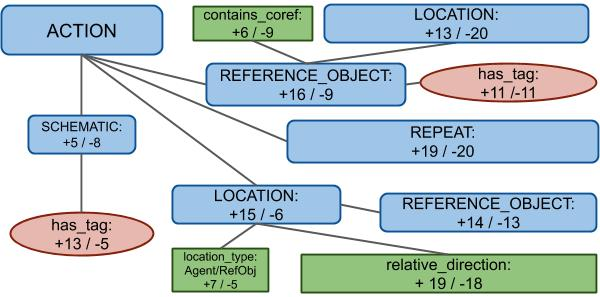
\includegraphics[width=\linewidth ]{figures/ModelMistakesNarrow.jpg}
    \caption{\label{fig:mistakes} We show nodes in the grammar which are most often wrongly predicted, with false positive (+) and false negative counts (-).}
\end{figure}

\paragraph{Error Analysis: } We further investigate the errors of the Seq2seq models on one of the data splits. We find that the model still struggles with span predictions: out of 363 errors, 125 only make mistakes on spans (and 199 get the tree structure right but make mistakes on leaves). Figure~\ref{fig:mistakes} shows the nodes which are most commonly mistaken, with the number of false positive and false negatives out of these 363 mistakes. Unsurprisingly, the most commonly confused span leaf is ``has\_tag'', which we use as a miscellaneous marker. Aside from that ``has\_tag'' however, the span mistakes are evenly spread over all other leaves. The next most common source of mistakes comes from the model struggling between identifying whether a provided location corresponds to the target of the action or to the reference object, and to identify instructions which imply a repetition. The former indicates a lack of compositionality in the input representation: the model correctly identifies that a location is mentioned, but fails to identify its context. Repeat conditions on the other hand challenge the model due to the wide variety of possible stop condition, a problem we suggest future work pay special attention to.

